\section{Verbale della riunione}
\subsection{Versionamento}
Nel ticket di Jira deve essere segnata la versione che corrisponde al lavoro. Lo scatto di versione avverrà al completamento della verifica.
\\Nuova tabella per il registro delle modifiche dei documenti:
\begin{figure}[H]
	\centering
	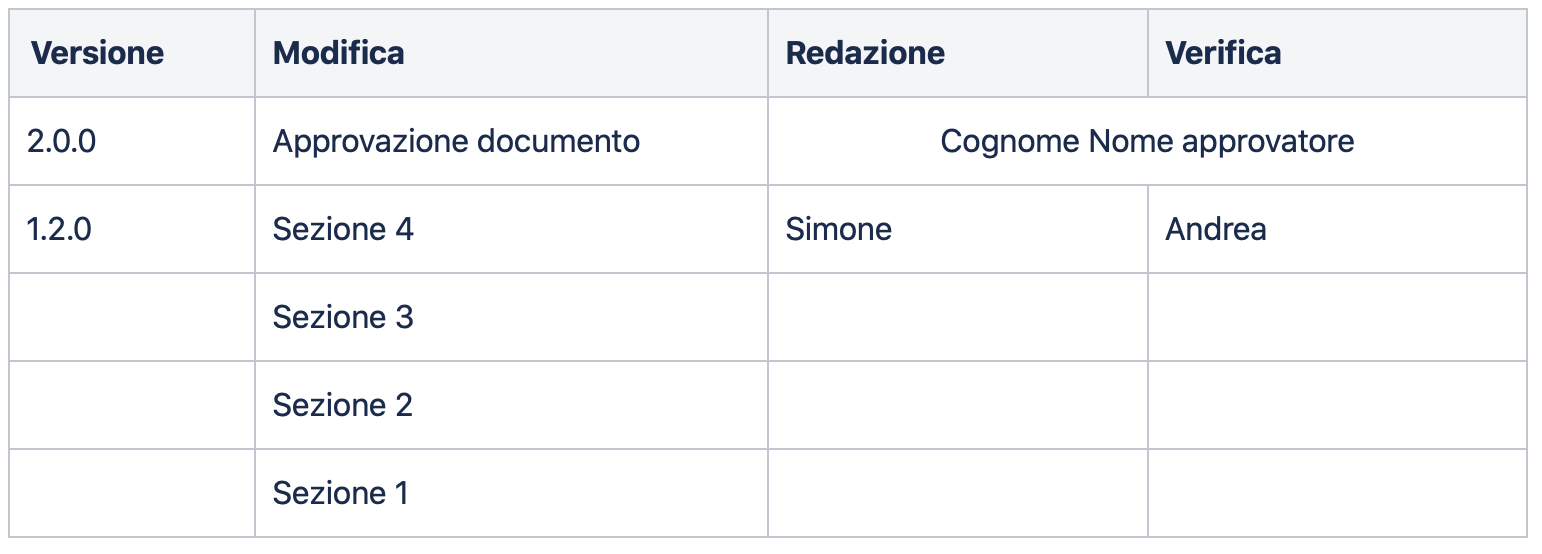
\includegraphics[scale=0.52]{res/images/tabella.png}
	\caption{esempio di nuova tabella per registro modifiche}
\end{figure}

\subsection{Glossario}
Dopo le correzioni si è deciso di apportare le seguenti modifiche al \textsc{Glossario}:
\begin{itemize}
	\item usare la wiki di GitHub per le definizioni dei termini;
	\item lo script inserirà nei documenti solo i pedici \textit{A} e \textit{G};
	\begin{itemize}
		\item il glossario proprio di ogni documento verrà cancellato;
	\end{itemize}
	\item nei riferimenti si inserirà il link alla wiki su GitHub;
	\item al momento del rilascio, la wiki sarà esportata in pdf.
\end{itemize}

\subsection{Piano di Qualifica}
\subsubsection{Possibili metriche}
Sono state individuate le seguenti metriche:
\begin{itemize}
	\item \textbf{durata delle riunioni}: rapporto tra durata prevista e durata effettiva;
	\item \textbf{indice di sincronizzazione}: rapporto tra tempo speso in riunioni asincrone e quello speso in totale da tutti;
	\item \textbf{rapporto tra tempo speso e tempo preventivato}: da segnare in un foglio Google Sheet;
	\item \textbf{uniformità dell'occupazione del tempo}: rapporta tra il totale delle ore spese diviso il numero dei partecipanti (6) e il totale delle ore di ogni singolo membro;
	\item \textbf{uniformità del lavoro nel tempo}: ogni giorno quanto ci si scosta dalla media dei ticket risolti nel periodo;
	\item \textbf{rispetto delle scadenze}: discostamento tra il completamento del lavoro rispetto alla scadenza fissata nella task;
	\item \textbf{budget variance};
	\item \textbf{schedule variance}.
\end{itemize}
\subsubsection{Tracciamento metriche}
Le metriche verranno tracciate in un foglio Google Sheet condiviso, dal quale è possibile generare grafici e calcoli automatici. Quando necessario si prenderà un'istantanea del cruscotto.

\subsection{Piano di Progetto}
Modifiche da consegnare alla RP:
\begin{itemize}
	\item trasformare le "fasi" in "periodi" che corrispondono alla divisione interna;
	\item lasciare la pianificazione a grana grossa in principio, ma aggiungere a cavallo tra due periodi una sezione per pianificare più in dettaglio le attività. Questa conterrà anche il preventivo a finire che sarà modificato rispetto a quello iniziale in base all'esperienza fatta; ogni preventivo dipende dal preventivo a finire precedente.
\end{itemize}

\subsection{Verbali}
Si è deciso di apportare le seguenti modifiche nella stesura dei verbali:
\begin{itemize}
	\item \textbf{Interni:}
	\begin{itemize}
		\item stesura più schematica, preferibile per punti elenco. Meno narrativi;
		\item tabella finale con il tracciamento dei temi affrontati (codice VI\_x.y).
	\end{itemize}
	\item \textbf{Esterni:} 
	\begin{itemize}
		\item struttura dell'incontro in domande e risposte, schematizzate in subsubsection. La descrizione deve essere più verbosa;
		\item tabella finale con il tracciamento delle domande con relative risposte (codice VE\_x.y).
	\end{itemize}
\end{itemize}

\subsection{Repository}
Sono state prese le seguenti decisioni per la gestione della \textit{repository} su GitHub:
\begin{itemize}
	\item eliminazione dei branch riguardandi la RR;
	\item rinominazione della cartella \textit{01\_RR} in \textit{documenti}. Questa contiene tutte le versioni dei documenti e per le revisioni si crea una \textit{release};
	\item sistemazione del template \LaTeX\ per la tabella del tracciamento delle modifiche \footnote{vedi sezione \S\ 2.1};
\end{itemize}
